\graphicspath{{chapters/contents/sessio_01/images/}}

\section{Sessió 01 (14/09/26). Continguts. Què és tot això de la ciència?}

Aquella nit de 1611, a Roma, un professor de matemàtiques anomenat \textbf{Galileu Galilei} segurament no devia poder aclucar gaire l’ull. L’endemà havia de plantar-se davant dels matemàtics i astrònoms jesuïtes del \textbf{Col·legi Romà}, alguns dels estudiosos més respectats del moment, i convèncer-los que allò que havia vist amb el seu telescopi era real. 

I el que havia vist no era poca cosa.

Tot havia començat un parell d’anys abans. El 1609, Galileu, que aleshores era professor de matemàtiques a la Universitat de Pàdua, s’havia assabentat que a Holanda havien construït un aparell capaç de fer veure més a prop els objectes llunyans. No en tenia cap, així que se’n va fabricar un. Després el va millorar. I un dia va decidir apuntar-lo al cel.



\begin{figure}[H]
    \centering
    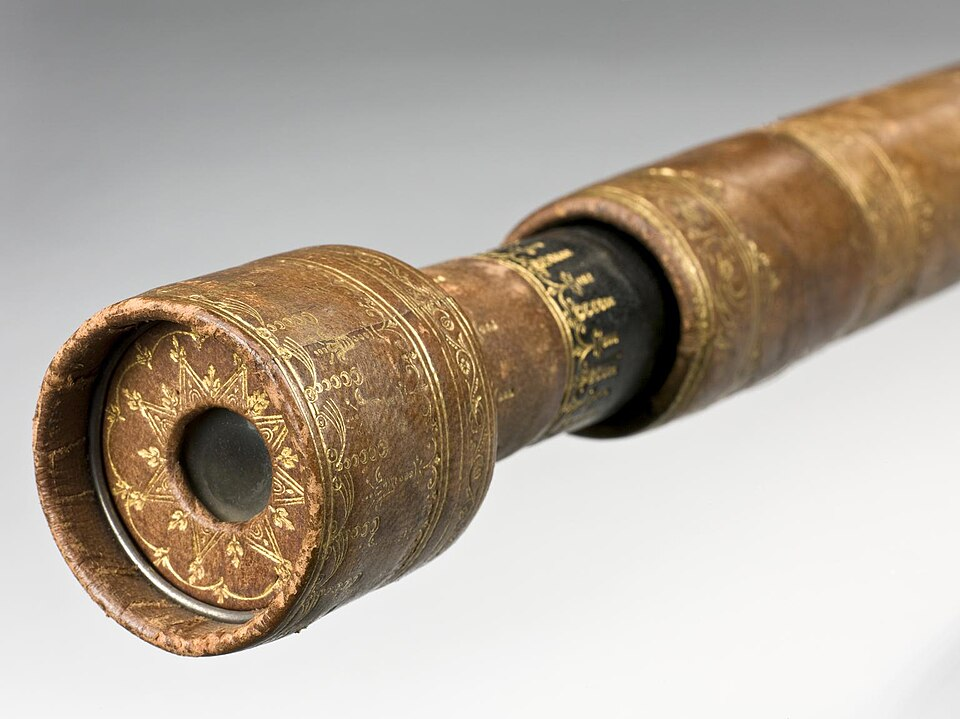
\includegraphics[width=0.75\linewidth]{telescopi_galileu.jpg}
    \caption{Telescopi de Galileu — Wikimedia Commons, CC BY 4.0.}
\end{figure}

Aquí és quan la cosa es va començar a complicar.

La Lluna tenia muntanyes i cràters, tot i que durant segles s’havia defensat que els cossos celestes havien de ser perfectes i sense irregularitats. Júpiter tenia quatre llunes girant al seu voltant, cosa que tampoc encaixava gaire bé amb la idea que absolutament tot havia de girar al voltant de la Terra.

El telescopi era una meravella. El problema començava quan tocava explicar què significava allò que s’hi veia.

I per entendre per què tot això va muntar tant de sarau, hem d’anar molt més enrere: fins al món antic i, en particular, a l’antiga Grècia.

\begin{figure}[H]
    \centering
    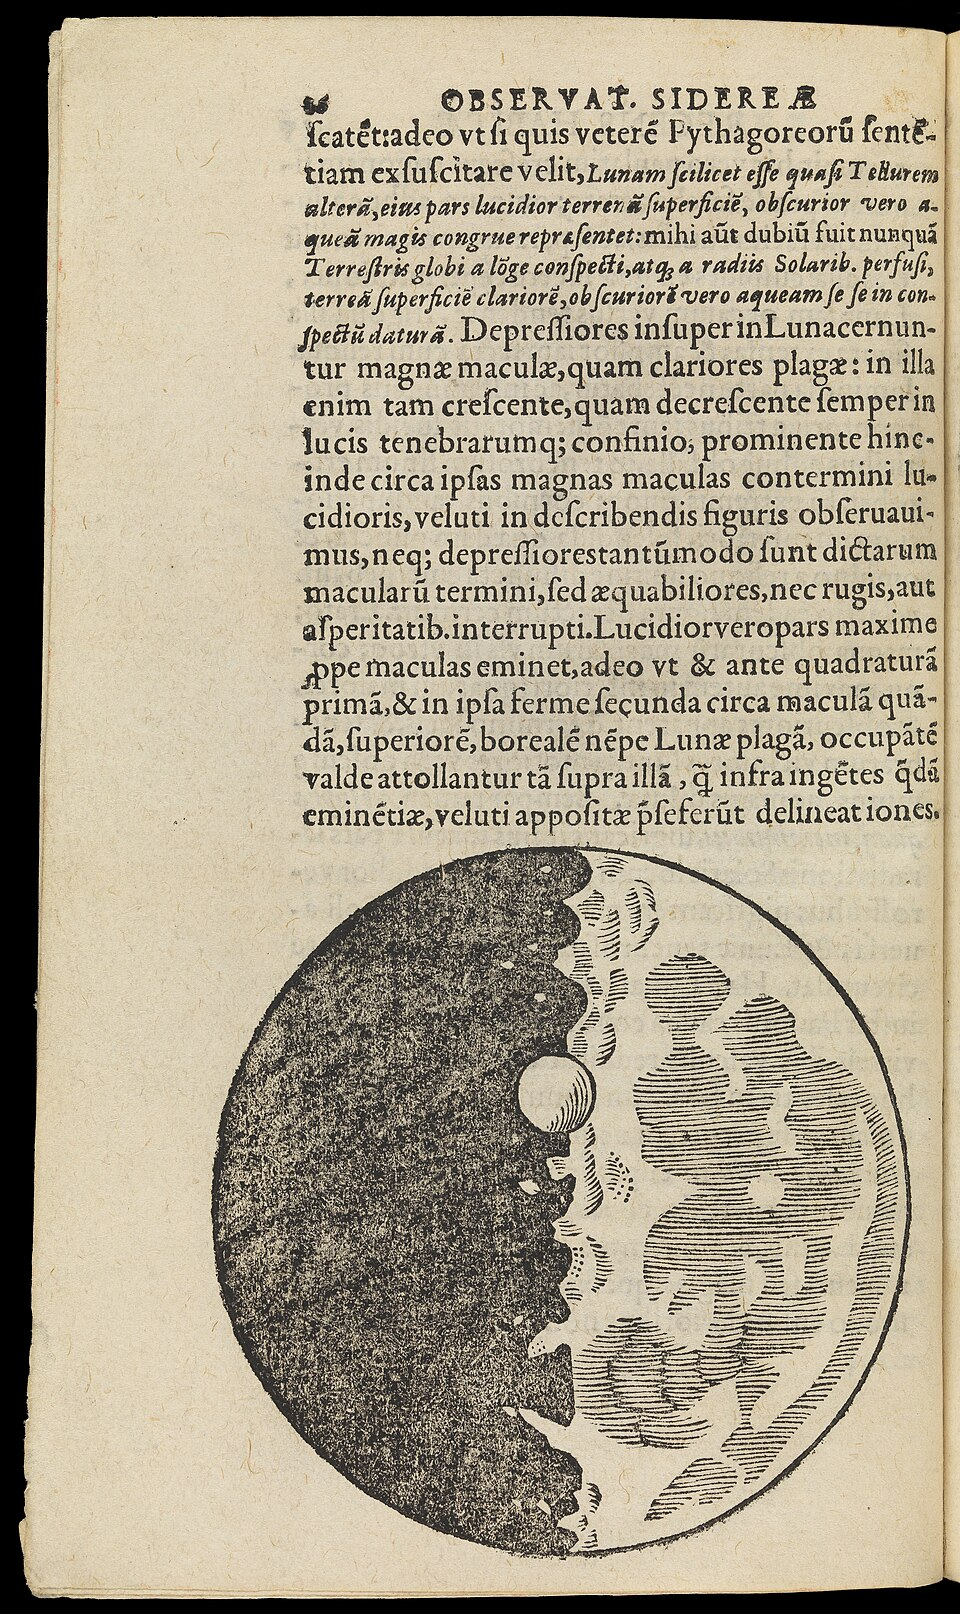
\includegraphics[width=0.75\linewidth]{sidereus_nuncius_lluna.jpg}
    \caption{Dibuix de la lluna fet et pel mateix Galileu.  Wikimedia Commons, CC BY 4.0.}
\end{figure}

Durant molt de temps, moltes coses del món s’havien explicat amb mites, déus i relats tradicionals. Però a la Grècia antiga alguns pensadors van començar a provar una altra via: observar la natura i preguntar-se si es podia explicar sense recórrer sempre a causes sobrenaturals.

Aristòtil no va ser el primer a fer-ho, però sí un dels primers a convertir aquesta manera de pensar en un sistema enorme i ordenat. La idea era, simplificant molt: mirem què passa, intentem raonar per què passa i construïm una explicació coherent. Durant segles, la seva influència va ser tan gran que moltes de les seves idees es van convertir gairebé en el punt de partida obligatori per pensar la natura.

I en unes quantes coses la va encertar: va defensar que la Terra era esfèrica, va estudiar i classificar animals i plantes i va entendre que valia la pena investigar la natura buscant-ne les causes.

Però també havia deixat algunes idees que, amb el temps, havien envellit regular:

\begin{itemize}
    \item els objectes pesants cauen més de pressa que els lleugers;
    \item la Terra roman immòbil al centre del cosmos;
    \item per mantenir un objecte en moviment cal continuar exercint-hi una força;
    \item tota la matèria terrestre està formada per quatre elements: terra, aigua, aire i foc.
\end{itemize}
El problema no era equivocar-se. Això ens passa a tots. El problema era com decidir quina explicació era correcta quan dues idees competien.

Aquí és on Galileu i altres autors van començar a canviar les regles del joc. Ja no n’hi havia prou que una explicació semblés raonable. Calia posar-la a prova:

\begin{itemize}
    \item observar;
    \item aïllar el fenomen mitjançant experiments;
    \item mesurar;
    \item utilitzar les matemàtiques quan fos possible;
    \item construir una explicació que es pogués contrastar amb noves observacions.
\end{itemize}

Si ho mirem bé, avui el procés és molt més complex, però continuem fent essencialment això: plantejar preguntes, recollir dades, construir models i comprovar si el que diem aguanta quan ho comparem amb la realitat.

Galileu va tenir bastants problemes per defensar l’heliocentrisme i el 1633 va ser obligat per la Inquisició a abjurar públicament de les seves idees i condemnat a arrest domiciliari. Però, per aquella època, la bola de neu de la \textbf{Revolució Científica} ja havia començat a rodolar muntanya avall.

Durant el segle XVII, Kepler, Galileu, Descartes, Newton i molts altres van anar construint una nova manera d’estudiar la natura. Newton va aconseguir reunir bona part d’aquestes peces en un sistema matemàtic capaç d’explicar des de la caiguda d’una pedra fins al moviment dels planetes.

Aquest procés és el que anomenem \textbf{Revolució Científica}. I bona part de la ciència que estudiarem aquest curs neix precisament aquí.

\section{La ciència moderna}

Fer ciència actualment és bastant més complicat que seguir quatre passos escrits en una llista, però es conserva una idea fonamental: intentar separar allò que pensem d’allò que podem comprovar.

Observem, mesurem, fem experiments, construïm models, discutim resultats i intentem que altres persones els puguin comprovar. Una explicació científica no ens ha de semblar bonica: ha de sobreviure a les proves.

\begin{figure}
    \centering
    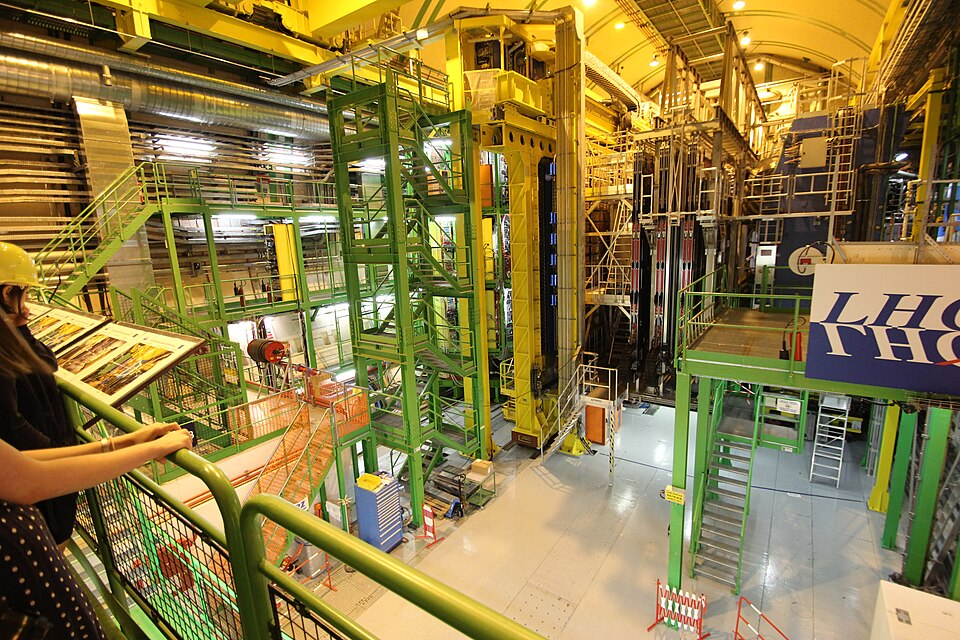
\includegraphics[width=0.75\linewidth]{cern_accelerador_particules.jpg}
    \caption{El CERN, a prop de Ginebra, és un dels grans centres mundials de recerca en física de partícules. Wikimedia Commons, CC BY 4.0.}
\end{figure}

També convé recordar algunes coses que els llibres acostumen a explicar bastant menys.

La ciència necessita diners. Els laboratoris costen, els instruments costen i aconseguir finançament forma part de la investigació pràcticament des del començament de la ciència.

Tampoc avança fent salts perfectament ordenats. Ens encanten els noms i les dates perquè fan que la història sigui manejable, però gairebé ningú es va llevar un matí dient: «Avui inventaré la química». Els descobriments es barregen, s’acumulen i sovint apareixen després de molts intents, discussions i errors.

I, sobretot, la ciència la fan persones. Hi ha científics brillants que van ser persones força discutibles, descobriments importants que van sorgir gairebé per accident i gent que va acabar revolucionant un camp al qual ni tan sols pensava dedicar-se. Aquesta part de la ciència també pot ser molt interessant i, de vegades, bastant divertida.

També ha estat una activitat profundament desigual. Durant segles, les dones van tenir moltes més dificultats per accedir a l’educació, les universitats i les institucions científiques, i moltes contribucions van ser ignorades, menystingudes o atribuïdes a altres persones.

Saber-ho no serveix només per mirar enrere: serveix per reconèixer aquestes barreres quan encara existeixen i per plantar-hi cara. Si alguna persona, sigui quina sigui la seva identitat, origen, capacitat o diversitat, arriba a pensar que la ciència «no és per a ella», aquí hi ha alguna cosa que s’està fent malament. La ciència necessita totes les mirades, totes les preguntes i tot el talent possible. Ha de ser, de debò, patrimoni de tota la humanitat.

\section{Què és la física?}

La física y la química totes dues estudien la natura, però posen el focus en problemes diferents.

La \textbf{física} intenta descriure algunes de les regles més generals de la natura. A l’ESO estudiarem sobretot física clàssica. No et preocupis si encara no ho entens tot: precisament som aquí per anar-ho descobrint.

\begin{itemize}
    \item moviment: posició, velocitat i acceleració;
    \item forces i causes del moviment;
    \item fluids: líquids i gasos;
    \item temperatura, calor i canvis d’energia;
    \item ones, llum i so;
    \item electricitat i magnetisme.
\end{itemize}
Entre tots aquests temes apareixerà contínuament una idea que els connecta: \textbf{l’energia}. Es pot emmagatzemar, transferir i transformar, i seguir-ne la pista permet entendre fenòmens que, a primera vista, semblen no tenir gaire cosa a veure entre si.

La física moderna entra en escena sobretot quan la física clàssica comença a quedar curta: en el món extremadament petit dels àtoms i les partícules, a velocitats pròximes a la de la llum o quan estudiem fenòmens a escala còsmica. Aquí les coses es compliquen bastant i les eines matemàtiques també pugen de nivell. Ja hi arribarem; de moment no cal córrer tant.

\section{Què és la química?}

La \textbf{química} s’ocupa principalment de què està feta la matèria i de com unes substàncies es poden transformar en unes altres.

La seva història va ser una mica més accidentada. Durant segles va estar barrejada amb l’alquímia, on convivien tècniques de laboratori molt útils amb objectius força ambiciosos, com fabricar or o trobar l’elixir de la vida eterna. La segona part va sortir regular; la primera va deixar aparells, substàncies i procediments que van ajudar a construir la química moderna.

El nostre camí començarà amb una pregunta aparentment senzilla: \textbf{si ningú no pot veure un àtom a simple vista, com sabem que existeix?}

A partir d’aquí, anirem \textbf{estirant el fil}:

\begin{itemize}
    \item els diferents models que hem utilitzat per descriure com és un àtom per dins i per què els hem hagut d’anar canviant amb el temps;
    \item els espectres i la taula periòdica, dues eines més que ens ajudaran a entendre millor com estan organitzats els àtoms i per què es comporten de maneres diferents;
    \item com s’uneixen els àtoms per formar substàncies, com escrivim fórmules per representar-les i com descrivim les reaccions que poden tenir lloc entre elles;
    \item algunes de les reaccions i processos químics més importants, com les dissolucions, les reaccions àcid-base o les d’oxidació-reducció;
    \item i, finalment, com apareix tot això fora del llibre: materials, aliments, medicaments, energia, indústria, contaminació i processos quotidians.
\end{itemize}
La idea no és col·leccionar fórmules i noms perquè sí. És aprendre a mirar un fenomen, separar allò important del soroll, mesurar el que puguem i construir una explicació que aguanti quan la posem a prova. Això, al final, és una definició força bona del que farem durant el curs.

